\documentclass[main.tex]{subfiles}
\begin{document}

\section{Discussion}
\subsection{On the nonsynthetic behaviour of the eigenstates}\label{sec:nonsynbeh}
Why is there such a sharp distinction between the nonsynthetic forces on the different fast
Hamiltonian eigenstates as seen in figure \ref{fig:ncompare}? This can be understood
in the limit \(J \ll \gamma\). For such parameters, which is often the case considered, the
eigenstates of the fast Hamiltonian will tend to the simple cases of \(\ket{\va{n}, 1}\),
\(\ket{\va{n}, 0}\) and \(\ket{\va{n}, -1}\), where the integer designates the directional
spin along the axis \(\va{n}\) of the external magnetic field. This follows from that the fast
Hamiltonian is diagonalizable at \(J = 0\), where the high and low energy states
in addition can be seen as the spin pointing in antiparallell or
parallel fashion, respectively, to the external field. The fast energies of those
states will tend towards \(-B\gamma\hbar{}\), \(0\) and \(B\gamma \hbar{}\) respectively.
The only quantity therein dependent on the position or angle of the dumbbell is the
external field strength \(B\), and since the nonsynthetic force acts in opposite direction
to the fast energy gradient the \textit{only} behaviour of the dumbbell in this limit is to
seek or avoid higher external field strengths, depending on whether the low or high energy
state is assumed. 

It is also the case that within the volume enclosed between the two coils, the lab,
external field strength is at its highest further away from the centre, close to the coils,
and at its lowest at the point of zero field magnitude at the centre. By this simple
reasoning it becomes clear that the high energy state will be attracted to the centre of
the lab, while the low energy state is quickly pushed away from that very point. The middle
state has no energy gradient in the limit of low \(J\), and so passes through the lab
without any nonsynthetic force acting on it.

\subsection{On the topic of mass}
It is a peculiar feature of the synthetic magnetic field that its strength is hardly
affected by the parameters of the setup. As discussed in section \ref{sec:resmiddle} for a
fixed magnetic field configuration this means adjustment of the dumbbell mass is a major
tool for exploring synthetic dynamics. For the middle state however these dynamics became
significant first when the mass was reduced to values in the order of \(\sim 10^{-29}\) kg, a
most displeasing result. The atomic mass unit is approximately \(1.66\times 10^{-27}\) kg, 
dumbbell masses but a hundredth of this magnitude are far from feasible for any system
where the movement can be considered ''slow'' and classical. Consequently the results
of section \ref{sec:resmiddle} may be considered of value mostly due to the appearance of the
predicted repulsive nature of the synthetic scalar field.

The case of the high energy states however bring great promise when it comes to domains of
mass. Not only is the synthetic effects visible for the dumbbell mass of two silver atoms,
rather heavy an element, but strong synthetic action appears already at masses in the order
of \(\sim 10^{-27}\). Diatomic dumbbells of light elements such as hydrogen lie within this
mass region, and as of such could constitute candidates for realisations of the model if
ever that enterprise is undertaken.

Adjustments of mass lead, at least in the high energy case, to corresponding adjustments of
the spin-field coupling strength \(\gamma B\) as was done in section  \ref{sec:reshigh}.
There, adjustments were only done to \(\gamma\), since field strength adjustments are
computationally more demanding, but it is of course the case that any real life realisation
of the system would carry with it some rather fixed value of \(\gamma\). It is therefore
fortunate that the field strength in a realisation is highly adjustable by means of the
current flowing through the coils. It remains unknown whether the currents needed are of
reasonable order, but this could be checked by estimating plausible dumbbell
parameters.

Is mass the \textit{only} tool available for strengthening the synthetic effects? This
need not be the case. Recalling the link between the Born-Oppenheimer synthetic magnetic
field and the geometric phase, it is clear that traversing larger swathes of
parameter space is connected to larger synthetic magnetic field action. This geometric line
of thinking can elucidate the independence of the synthetic fields on energy magnitudes.
Increasing the energy magnitudes, say through increasing \(B\), does not change the
path taken through parameter space more than multiplying its distance to the origin.
Typical geometric phases, such as Berry's initial consideration of a system like that
discussed in
section \ref{sec:adiab}, are independent of the path's distance to the origin, and by these
means the energy magnitudes can be seen to not affect the synthetic magnetic field effects.

Here, another way of strengthening the synthetic effects become clear: by complicating the
path taken through parameter space. The capability of the dumbbell to rotate already
constitute a great achievement in this regard, as the relative direction of the magnetic
field to the dumbbell axis may vary much more than what would otherwise be the case.
Something not done here is however letting the dumbbell pass through some much more
complicated external field. Many options are here available with nothing but one's
creativity setting the limits. A more complicated field does however also complicate the
study of the monopoles in the synthetic field, as the complexity of the mapping between
real space and parameter space increases.

\subsection{On the topic of monopoles}
It was an explicit objective of this project to study the dynamics arising from magnetic monopole
fields, as these are made available by the synthetic magnetic field. While non-negligible
synthetic field action has been demonstrated for both the synthetic scalar and magnetic
field, most prominently in the simulations of figure \ref{fig:n2m-27A}, the interpretation
of these fields as arising from monopole action is a difficult one to consider. 

One reason for such difficulties is simply that the monopoles to the synthetic magnetic
field ''live'' in the appropriate parameter space, in the present case the space of
external fields, both when it comes to their locations as
well as the field they generate. 
%The Lorentz-type force due to the synthetic field however
%acts in real space, and since the mapping between the real and parameter spaces are not
%identity, in general it is rather nontrivial, there exists a fatal mismatch. If monopole
%fields are to be studied as they would act in the case of fundamental magnetic monopoles
%the motion through parameter space, i.e. through the synthetic magnetic field seen as generated
%by monopoles, should look as if affected by that very field. The forces now act however on
%the motion through real space, and will therefore in general \textit{not} have the correct
%direction when transformed into parameter space. The complexity of this argument warrants
%an example. For the case of \(J=0\), that is the system of section \ref{sec:adiab} as
%studied by Berry, the synthetic field in parameter space is generated by a monopole at the
%origin. Consider then the dumbbell moving in the positive \(z\) direction in the
%\(zx\) plane through parameter space. %%Okej tror inte riktigt jag förstår det här, fråga
%%Erik?
The map between this space and real space cannot however be  the identity map, such an external
field is not allowed by Maxwell's equations,  instead the map will be rather nontrivial in general.
Any motion through real space must therefore first be ''translated'' by means of this map
if that motion is to be seen as motion in a monopole field. Luckily the present choice of
external magnetic field inadvertently implies a not too complex such map, see figure
\ref{fig:fieldcompare}. As described in
section \ref{sec:chofield} the external field from the two opposing coils increase in
magnitude with increasing distance to the zero-point at the centre. The field additionally
points towards the \(xy\)-plane intersecting the centre, and points either away
from or towards the axis of symmetry depending on the choice of current direction.
Therefore a simple reflection in the mentioned \(xy\)-plane followed, if the current
direction requires it, by inversions of the \(x\) and \(y\) coordinates about the centre is
almost the map between real space and parameter space required. Some scaling of all
dimensions must also be performed, the details of which are potentially quite complex.
%Jag är väldigt osäker på den här diskussionen, om transformationen mellan reell och
%parameter ens behövs

\begin{figure}[h]
        \centering
        \begin{tikzpicture}
                \draw[black]
                        (-4, 0) node{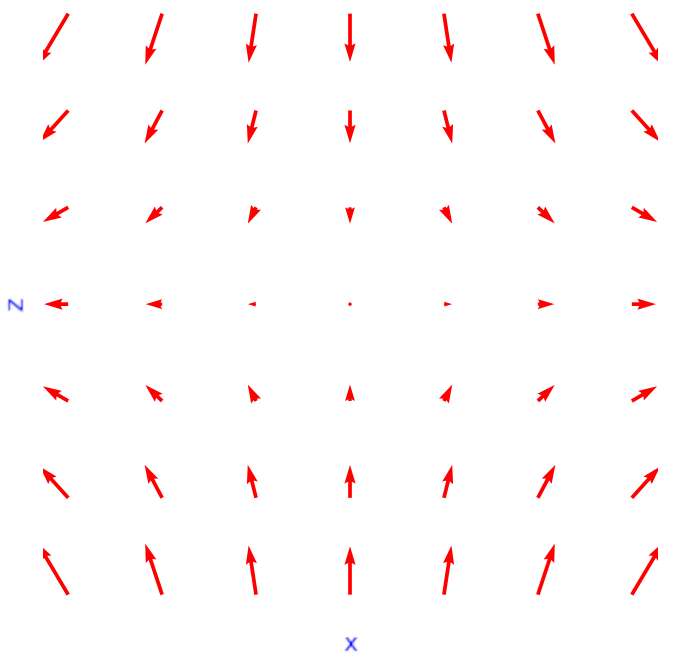
\includegraphics[width=0.3\textwidth]{figures/coilfield-e}};
                \draw[black] (-3.9,-2.8) node{External field in real space.};
                \draw[black, ->] (-1,0) to[out=30, in=150] (1,0);
                \draw[black] (0,0.7) node{\(M\) };
                \draw[black]
                        (4, 0)node[yshift=0.4]{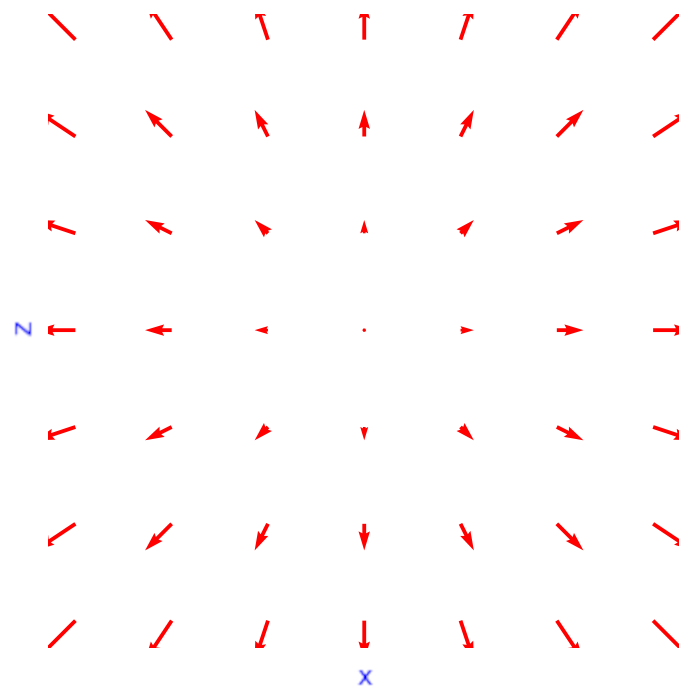
\includegraphics[width=0.29\textwidth]{figures/idealfield-e}};
                \draw[black] (4.1,-2.8) node{External field in parameter space.};
        \end{tikzpicture}
        \caption{\centering An illustration of the map \(M\) between real space and parameter space,
        which must map every point of external field \(\va{b}\) to the parameter space
point with the same external field \(\va{b}\). The planes shown are the \(xz\)-planes
through the zero-field centre point of the lab and the origin, respectively.}
        \label{fig:fieldcompare}
\end{figure}

It can also be noted, in contrast with the established goal, that the modification of the
pure monopolar magnetic synthetic field by the introduction of the spin-spin coupling
breaks the monopolar structure in unwanted ways. While the splitting of magnetic charge as
described in section \ref{sec:regmono} is desired and interesting, it is also associated
with a conversion of the field from purely monopolar to a field of nonzero curl. If we wish
to study the effects of the monopole action this will obscure the results with dynamics
arising from the non-monopolar part of the field, and separating the two effects may be
impossible.

\subsection{Numerical limitations}
While the scripts written appear to work as intended no real analysis of their errors and
stability has been performed. The apparent instability of the results presented in section
\ref{sec:resmiddle} in particular motivate such considerations. The division of the lab into a discrete lattice, as well as
the discretization of dumbbell rotation angles, can be assumed to limit the accuracy of the
result. The selection of \(101^3\) sites in the lattice was merely due to performance
limitations, that number would have been increased had the setup allowed it, but the external
field generation function quickly ran out of available resources if this was trialled. The
discussion of section \ref{sec:code} shows that the used granularity is far below the
optimal selection for the performance of the numerical differentiations, so increasing the
amount of sites would be of high priority were the code to be optimized further.

It was also encountered that the ODE solver simply would not converge in any
reasonable amount of time for many
choices of parameters. Being highly undesirable since this narrows the parameter ranges available
for study, the precise reasons for this behaviour warrants further investigation. As an
example large values of \(J\) or reductions of the dumbbell length \(l\) would often not
integrate properly as the rotational accelerations and velocities became exceedingly large.
Fast rotation of the dumbbell is perhaps not unphysical for the scenario considered, but
appeared to not behave well in the numerical simulation. In addition it will be noted that
exceedingly quick rotation could violate the adiabatic approximation, undermining the
model. A possible correction to the model, if such rotations are deemed physical, could be to consider
the rotational degrees of freedom part of the fast system instead of the slow. A hypothesis considering the origin of these non-convergent parameters is that the
ODE solver does not behave well in conjunction with the lab discretization. The solver
wishes to keep certain error estimates below a threshold value, here set to depend on the
granularity of the lattice, and will reduce the step size of the integration until this is
satisfied. It could be the case however that reductions of step size do not yield the
intended effect for the solver, as the fitting of all positions to points in the lattice
puts a lower bound on the effective step size attainable. Further investigation would be
desirable.
\end{document}
